\documentclass[twoside]{book}

% Packages required by doxygen
\usepackage{fixltx2e}
\usepackage{calc}
\usepackage{doxygen}
\usepackage[export]{adjustbox} % also loads graphicx
\usepackage{graphicx}
\usepackage[utf8]{inputenc}
\usepackage{makeidx}
\usepackage{multicol}
\usepackage{multirow}
\PassOptionsToPackage{warn}{textcomp}
\usepackage{textcomp}
\usepackage[nointegrals]{wasysym}
\usepackage[table]{xcolor}

% Font selection
\usepackage[T1]{fontenc}
\usepackage[scaled=.90]{helvet}
\usepackage{courier}
\usepackage{amssymb}
\usepackage{sectsty}
\renewcommand{\familydefault}{\sfdefault}
\allsectionsfont{%
  \fontseries{bc}\selectfont%
  \color{darkgray}%
}
\renewcommand{\DoxyLabelFont}{%
  \fontseries{bc}\selectfont%
  \color{darkgray}%
}
\newcommand{\+}{\discretionary{\mbox{\scriptsize$\hookleftarrow$}}{}{}}

% Page & text layout
\usepackage{geometry}
\geometry{%
  a4paper,%
  top=2.5cm,%
  bottom=2.5cm,%
  left=2.5cm,%
  right=2.5cm%
}
\tolerance=750
\hfuzz=15pt
\hbadness=750
\setlength{\emergencystretch}{15pt}
\setlength{\parindent}{0cm}
\setlength{\parskip}{3ex plus 2ex minus 2ex}
\makeatletter
\renewcommand{\paragraph}{%
  \@startsection{paragraph}{4}{0ex}{-1.0ex}{1.0ex}{%
    \normalfont\normalsize\bfseries\SS@parafont%
  }%
}
\renewcommand{\subparagraph}{%
  \@startsection{subparagraph}{5}{0ex}{-1.0ex}{1.0ex}{%
    \normalfont\normalsize\bfseries\SS@subparafont%
  }%
}
\makeatother

% Headers & footers
\usepackage{fancyhdr}
\pagestyle{fancyplain}
\fancyhead[LE]{\fancyplain{}{\bfseries\thepage}}
\fancyhead[CE]{\fancyplain{}{}}
\fancyhead[RE]{\fancyplain{}{\bfseries\leftmark}}
\fancyhead[LO]{\fancyplain{}{\bfseries\rightmark}}
\fancyhead[CO]{\fancyplain{}{}}
\fancyhead[RO]{\fancyplain{}{\bfseries\thepage}}
\fancyfoot[LE]{\fancyplain{}{}}
\fancyfoot[CE]{\fancyplain{}{}}
\fancyfoot[RE]{\fancyplain{}{\bfseries\scriptsize Generated by Doxygen }}
\fancyfoot[LO]{\fancyplain{}{\bfseries\scriptsize Generated by Doxygen }}
\fancyfoot[CO]{\fancyplain{}{}}
\fancyfoot[RO]{\fancyplain{}{}}
\renewcommand{\footrulewidth}{0.4pt}
\renewcommand{\chaptermark}[1]{%
  \markboth{#1}{}%
}
\renewcommand{\sectionmark}[1]{%
  \markright{\thesection\ #1}%
}

% Indices & bibliography
\usepackage{natbib}
\usepackage[titles]{tocloft}
\setcounter{tocdepth}{3}
\setcounter{secnumdepth}{5}
\makeindex

% Hyperlinks (required, but should be loaded last)
\usepackage{ifpdf}
\ifpdf
  \usepackage[pdftex,pagebackref=true]{hyperref}
\else
  \usepackage[ps2pdf,pagebackref=true]{hyperref}
\fi
\hypersetup{%
  colorlinks=true,%
  linkcolor=blue,%
  citecolor=blue,%
  unicode%
}

% Custom commands
\newcommand{\clearemptydoublepage}{%
  \newpage{\pagestyle{empty}\cleardoublepage}%
}

\usepackage{caption}
\captionsetup{labelsep=space,justification=centering,font={bf},singlelinecheck=off,skip=4pt,position=top}

%===== C O N T E N T S =====

\begin{document}

% Titlepage & ToC
\hypersetup{pageanchor=false,
             bookmarksnumbered=true,
             pdfencoding=unicode
            }
\pagenumbering{roman}
\begin{titlepage}
\vspace*{7cm}
\begin{center}%
{\Large Smart\+Compiler }\\
\vspace*{1cm}
{\large Generated by Doxygen 1.8.11}\\
\end{center}
\end{titlepage}
\clearemptydoublepage
\tableofcontents
\clearemptydoublepage
\pagenumbering{arabic}
\hypersetup{pageanchor=true}

%--- Begin generated contents ---
\chapter{Hierarchical Index}
\section{Class Hierarchy}
This inheritance list is sorted roughly, but not completely, alphabetically\+:\begin{DoxyCompactList}
\item \contentsline{section}{Util\+:\+:Config\+Reader}{\pageref{class_util_1_1_config_reader}}{}
\item \contentsline{section}{Util\+:\+:Environment}{\pageref{class_util_1_1_environment}}{}
\item \contentsline{section}{Util\+:\+:Message\+Mgr}{\pageref{class_util_1_1_message_mgr}}{}
\item \contentsline{section}{Util\+:\+:Message\+Type}{\pageref{struct_util_1_1_message_type}}{}
\item \contentsline{section}{Parser\+:\+:Parser\+ST}{\pageref{class_parser_1_1_parser_s_t}}{}
\item \contentsline{section}{Scanner\+:\+:Scanner\+ST}{\pageref{class_scanner_1_1_scanner_s_t}}{}
\item \contentsline{section}{Scanner\+:\+:Source\+File}{\pageref{class_scanner_1_1_source_file}}{}
\item Test\+Fixture\begin{DoxyCompactList}
\item \contentsline{section}{Parser\+:\+:Parser\+Test}{\pageref{class_parser_1_1_parser_test}}{}
\item \contentsline{section}{Scanner\+:\+:Scanner\+Test}{\pageref{class_scanner_1_1_scanner_test}}{}
\item \contentsline{section}{Util\+:\+:Util\+Test}{\pageref{class_util_1_1_util_test}}{}
\end{DoxyCompactList}
\item \contentsline{section}{Scanner\+:\+:Token}{\pageref{class_scanner_1_1_token}}{}
\begin{DoxyCompactList}
\item \contentsline{section}{Scanner\+:\+:Eof\+Token}{\pageref{class_scanner_1_1_eof_token}}{}
\item \contentsline{section}{Scanner\+:\+:Error\+Token}{\pageref{class_scanner_1_1_error_token}}{}
\item \contentsline{section}{Scanner\+:\+:Identifier\+Token}{\pageref{class_scanner_1_1_identifier_token}}{}
\item \contentsline{section}{Scanner\+:\+:Number\+Token}{\pageref{class_scanner_1_1_number_token}}{}
\item \contentsline{section}{Scanner\+:\+:Special\+Symbol\+Token}{\pageref{class_scanner_1_1_special_symbol_token}}{}
\end{DoxyCompactList}
\item \contentsline{section}{Parser\+:\+:Tree\+Node}{\pageref{class_parser_1_1_tree_node}}{}
\end{DoxyCompactList}

\chapter{Class Index}
\section{Class List}
Here are the classes, structs, unions and interfaces with brief descriptions\+:\begin{DoxyCompactList}
\item\contentsline{section}{\hyperlink{class_util_1_1_logger}{Util\+::\+Logger} }{\pageref{class_util_1_1_logger}}{}
\item\contentsline{section}{\hyperlink{class_scanner_1_1_scanner_s_t}{Scanner\+::\+Scanner\+ST} }{\pageref{class_scanner_1_1_scanner_s_t}}{}
\item\contentsline{section}{\hyperlink{class_scanner_test}{Scanner\+Test} }{\pageref{class_scanner_test}}{}
\item\contentsline{section}{\hyperlink{class_scanner_1_1_source_file}{Scanner\+::\+Source\+File} }{\pageref{class_scanner_1_1_source_file}}{}
\item\contentsline{section}{\hyperlink{class_scanner_1_1_token}{Scanner\+::\+Token} }{\pageref{class_scanner_1_1_token}}{}
\item\contentsline{section}{\hyperlink{class_util_1_1_util_test}{Util\+::\+Util\+Test} }{\pageref{class_util_1_1_util_test}}{}
\end{DoxyCompactList}

\chapter{Class Documentation}
\hypertarget{class_util_1_1_config_reader}{}\section{Util\+:\+:Config\+Reader Class Reference}
\label{class_util_1_1_config_reader}\index{Util\+::\+Config\+Reader@{Util\+::\+Config\+Reader}}
\subsection*{Public Member Functions}
\begin{DoxyCompactItemize}
\item 
\hyperlink{class_util_1_1_config_reader_a2b1191216e59d393f6bba458fdd664b3}{Config\+Reader} ()
\item 
\hyperlink{class_util_1_1_config_reader_ae8511b54dd87d3c740553852f2d562d1}{$\sim$\+Config\+Reader} ()
\item 
void \hyperlink{class_util_1_1_config_reader_a2b2fed9a1426e4f13dcd444ea96d2e71}{read\+Config\+File} (std\+::string \&)  throw (std\+::runtime\+\_\+error)
\item 
char $\ast$ {\bfseries get\+OptionA} ()\hypertarget{class_util_1_1_config_reader_a323932bdac00da4f6b354e8c5e17a8d1}{}\label{class_util_1_1_config_reader_a323932bdac00da4f6b354e8c5e17a8d1}

\end{DoxyCompactItemize}


\subsection{Constructor \& Destructor Documentation}
\index{Util\+::\+Config\+Reader@{Util\+::\+Config\+Reader}!Config\+Reader@{Config\+Reader}}
\index{Config\+Reader@{Config\+Reader}!Util\+::\+Config\+Reader@{Util\+::\+Config\+Reader}}
\subsubsection[{\texorpdfstring{Config\+Reader()}{ConfigReader()}}]{\setlength{\rightskip}{0pt plus 5cm}Util\+::\+Config\+Reader\+::\+Config\+Reader (
\begin{DoxyParamCaption}
{}
\end{DoxyParamCaption}
)}\hypertarget{class_util_1_1_config_reader_a2b1191216e59d393f6bba458fdd664b3}{}\label{class_util_1_1_config_reader_a2b1191216e59d393f6bba458fdd664b3}
Constructor initializes xerces-\/C libraries. The X\+ML tags and attributes which we seek are defined. The xerces-\/C D\+OM parser infrastructure is initialized. \index{Util\+::\+Config\+Reader@{Util\+::\+Config\+Reader}!````~Config\+Reader@{$\sim$\+Config\+Reader}}
\index{````~Config\+Reader@{$\sim$\+Config\+Reader}!Util\+::\+Config\+Reader@{Util\+::\+Config\+Reader}}
\subsubsection[{\texorpdfstring{$\sim$\+Config\+Reader()}{~ConfigReader()}}]{\setlength{\rightskip}{0pt plus 5cm}Util\+::\+Config\+Reader\+::$\sim$\+Config\+Reader (
\begin{DoxyParamCaption}
{}
\end{DoxyParamCaption}
)}\hypertarget{class_util_1_1_config_reader_ae8511b54dd87d3c740553852f2d562d1}{}\label{class_util_1_1_config_reader_ae8511b54dd87d3c740553852f2d562d1}
Class destructor frees memory used to hold the X\+ML tag and attribute definitions. It als terminates use of the xerces-\/C framework. 

\subsection{Member Function Documentation}
\index{Util\+::\+Config\+Reader@{Util\+::\+Config\+Reader}!read\+Config\+File@{read\+Config\+File}}
\index{read\+Config\+File@{read\+Config\+File}!Util\+::\+Config\+Reader@{Util\+::\+Config\+Reader}}
\subsubsection[{\texorpdfstring{read\+Config\+File(std\+::string \&)}{readConfigFile(std::string &)}}]{\setlength{\rightskip}{0pt plus 5cm}void Util\+::\+Config\+Reader\+::read\+Config\+File (
\begin{DoxyParamCaption}
\item[{std\+::string \&}]{}
\end{DoxyParamCaption}
) throw  std\+::runtime\+\_\+error) }\hypertarget{class_util_1_1_config_reader_a2b2fed9a1426e4f13dcd444ea96d2e71}{}\label{class_util_1_1_config_reader_a2b2fed9a1426e4f13dcd444ea96d2e71}
This function\+:
\begin{DoxyItemize}
\item Tests the access and availability of the X\+ML configuration file.
\item Configures the xerces-\/c D\+OM parser.
\item Reads and extracts the pertinent information from the X\+ML config file.
\end{DoxyItemize}


\begin{DoxyParams}{Parameters}
{\em in} & config\+File The text string name of the H\+LA configuration file. \\
\hline
\end{DoxyParams}


The documentation for this class was generated from the following files\+:\begin{DoxyCompactItemize}
\item 
Util/Config\+Reader.\+h\item 
Util/Config\+Reader.\+cpp\end{DoxyCompactItemize}

\hypertarget{class_util_1_1_environment}{}\section{Util\+:\+:Environment Class Reference}
\label{class_util_1_1_environment}\index{Util\+::\+Environment@{Util\+::\+Environment}}
\subsection*{Public Member Functions}
\begin{DoxyCompactItemize}
\item 
\hyperlink{class_util_1_1_message_mgr}{Message\+Mgr} \& {\bfseries get\+Message\+Mgr} ()\hypertarget{class_util_1_1_environment_aeabf16ed6959da86effea699c19b79f5}{}\label{class_util_1_1_environment_aeabf16ed6959da86effea699c19b79f5}

\item 
std\+::string {\bfseries get\+Cur\+Time} ()\hypertarget{class_util_1_1_environment_ae193832a3b616c6608bc0b89852bb656}{}\label{class_util_1_1_environment_ae193832a3b616c6608bc0b89852bb656}

\item 
std\+::string {\bfseries get\+Cur\+Working\+Dir} ()\hypertarget{class_util_1_1_environment_ae6c30571579f59b4fe149b90387bf864}{}\label{class_util_1_1_environment_ae6c30571579f59b4fe149b90387bf864}

\end{DoxyCompactItemize}
\subsection*{Static Public Member Functions}
\begin{DoxyCompactItemize}
\item 
static \hyperlink{class_util_1_1_environment}{Environment} \& {\bfseries get\+Environment} ()\hypertarget{class_util_1_1_environment_a9a0f53217764e53a1169422b0d3fc6fe}{}\label{class_util_1_1_environment_a9a0f53217764e53a1169422b0d3fc6fe}

\end{DoxyCompactItemize}


The documentation for this class was generated from the following files\+:\begin{DoxyCompactItemize}
\item 
Util/Environment.\+h\item 
Util/Environment.\+cpp\end{DoxyCompactItemize}

\hypertarget{class_scanner_1_1_eof_token}{}\section{Scanner\+:\+:Eof\+Token Class Reference}
\label{class_scanner_1_1_eof_token}\index{Scanner\+::\+Eof\+Token@{Scanner\+::\+Eof\+Token}}


Inheritance diagram for Scanner\+:\+:Eof\+Token\+:
\nopagebreak
\begin{figure}[H]
\begin{center}
\leavevmode
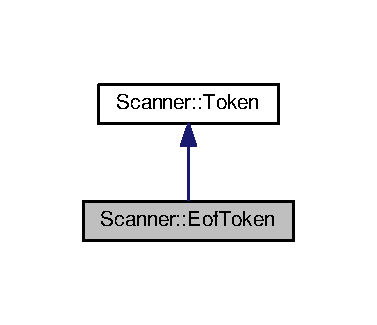
\includegraphics[width=181pt]{class_scanner_1_1_eof_token__inherit__graph}
\end{center}
\end{figure}


Collaboration diagram for Scanner\+:\+:Eof\+Token\+:
\nopagebreak
\begin{figure}[H]
\begin{center}
\leavevmode
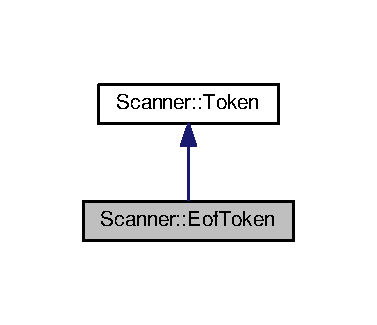
\includegraphics[width=181pt]{class_scanner_1_1_eof_token__coll__graph}
\end{center}
\end{figure}
\subsection*{Public Member Functions}
\begin{DoxyCompactItemize}
\item 
virtual void {\bfseries scan\+Token} (\hyperlink{class_scanner_1_1_source_file}{Source\+File} \&r\+File)\hypertarget{class_scanner_1_1_eof_token_a983b7417f05df2468fba9652f969d6c4}{}\label{class_scanner_1_1_eof_token_a983b7417f05df2468fba9652f969d6c4}

\end{DoxyCompactItemize}
\subsection*{Additional Inherited Members}


The documentation for this class was generated from the following files\+:\begin{DoxyCompactItemize}
\item 
Scanner/Eof\+Token.\+h\item 
Scanner/Eof\+Token.\+cpp\end{DoxyCompactItemize}

\hypertarget{class_scanner_1_1_error_token}{}\section{Scanner\+:\+:Error\+Token Class Reference}
\label{class_scanner_1_1_error_token}\index{Scanner\+::\+Error\+Token@{Scanner\+::\+Error\+Token}}


Inheritance diagram for Scanner\+:\+:Error\+Token\+:
\nopagebreak
\begin{figure}[H]
\begin{center}
\leavevmode
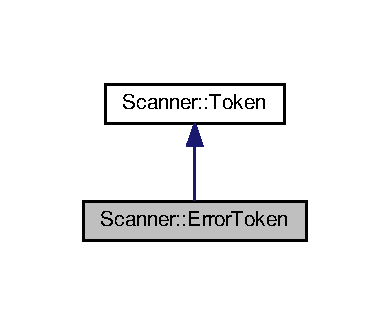
\includegraphics[width=187pt]{class_scanner_1_1_error_token__inherit__graph}
\end{center}
\end{figure}


Collaboration diagram for Scanner\+:\+:Error\+Token\+:
\nopagebreak
\begin{figure}[H]
\begin{center}
\leavevmode
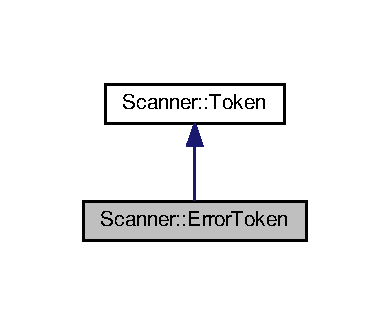
\includegraphics[width=187pt]{class_scanner_1_1_error_token__coll__graph}
\end{center}
\end{figure}
\subsection*{Public Member Functions}
\begin{DoxyCompactItemize}
\item 
virtual void {\bfseries scan\+Token} (\hyperlink{class_scanner_1_1_source_file}{Source\+File} \&r\+File)\hypertarget{class_scanner_1_1_error_token_a71999afcaec23264d91e8bc152de00bd}{}\label{class_scanner_1_1_error_token_a71999afcaec23264d91e8bc152de00bd}

\end{DoxyCompactItemize}
\subsection*{Additional Inherited Members}


The documentation for this class was generated from the following files\+:\begin{DoxyCompactItemize}
\item 
Scanner/Error\+Token.\+h\item 
Scanner/Error\+Token.\+cpp\end{DoxyCompactItemize}

\hypertarget{class_scanner_1_1_identifier_token}{}\section{Scanner\+:\+:Identifier\+Token Class Reference}
\label{class_scanner_1_1_identifier_token}\index{Scanner\+::\+Identifier\+Token@{Scanner\+::\+Identifier\+Token}}


Inheritance diagram for Scanner\+:\+:Identifier\+Token\+:
\nopagebreak
\begin{figure}[H]
\begin{center}
\leavevmode
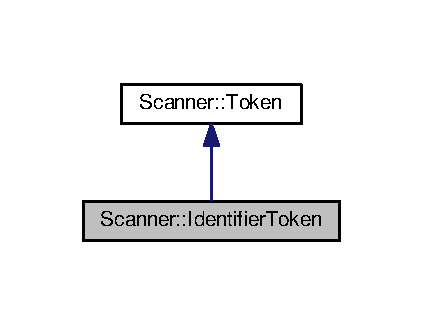
\includegraphics[width=203pt]{class_scanner_1_1_identifier_token__inherit__graph}
\end{center}
\end{figure}


Collaboration diagram for Scanner\+:\+:Identifier\+Token\+:
\nopagebreak
\begin{figure}[H]
\begin{center}
\leavevmode
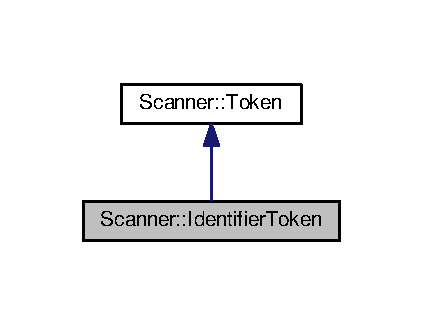
\includegraphics[width=203pt]{class_scanner_1_1_identifier_token__coll__graph}
\end{center}
\end{figure}
\subsection*{Public Member Functions}
\begin{DoxyCompactItemize}
\item 
virtual void {\bfseries scan\+Token} (\hyperlink{class_scanner_1_1_source_file}{Source\+File} \&r\+File)\hypertarget{class_scanner_1_1_identifier_token_a3fb2da988de14bc2f33d96e66efc18da}{}\label{class_scanner_1_1_identifier_token_a3fb2da988de14bc2f33d96e66efc18da}

\end{DoxyCompactItemize}
\subsection*{Additional Inherited Members}


The documentation for this class was generated from the following files\+:\begin{DoxyCompactItemize}
\item 
Scanner/Identifier\+Token.\+h\item 
Scanner/Identifier\+Token.\+cpp\end{DoxyCompactItemize}

\hypertarget{class_util_1_1_message_mgr}{}\section{Util\+:\+:Message\+Mgr Class Reference}
\label{class_util_1_1_message_mgr}\index{Util\+::\+Message\+Mgr@{Util\+::\+Message\+Mgr}}
\subsection*{Public Member Functions}
\begin{DoxyCompactItemize}
\item 
void {\bfseries init\+Message\+Mgr} (const string \&file\+Name)\hypertarget{class_util_1_1_message_mgr_a81f18324b306dc02210ca2335ee6592c}{}\label{class_util_1_1_message_mgr_a81f18324b306dc02210ca2335ee6592c}

\item 
void \hyperlink{class_util_1_1_message_mgr_ad50ef26d52890416645bb779926fed8d}{publish\+Message} (const Message\+Type\+::\+ID msg\+Type, const char $\ast$format,...)
\begin{DoxyCompactList}\small\item\em Publish given message with given format and parameters (variadic) \end{DoxyCompactList}\end{DoxyCompactItemize}


\subsection{Member Function Documentation}
\index{Util\+::\+Message\+Mgr@{Util\+::\+Message\+Mgr}!publish\+Message@{publish\+Message}}
\index{publish\+Message@{publish\+Message}!Util\+::\+Message\+Mgr@{Util\+::\+Message\+Mgr}}
\subsubsection[{\texorpdfstring{publish\+Message(const Message\+Type\+::\+I\+D msg\+Type, const char $\ast$format,...)}{publishMessage(const MessageType::ID msgType, const char *format,...)}}]{\setlength{\rightskip}{0pt plus 5cm}void Util\+::\+Message\+Mgr\+::publish\+Message (
\begin{DoxyParamCaption}
\item[{const Message\+Type\+::\+ID}]{msg\+Type, }
\item[{const char $\ast$}]{format, }
\item[{}]{...}
\end{DoxyParamCaption}
)}\hypertarget{class_util_1_1_message_mgr_ad50ef26d52890416645bb779926fed8d}{}\label{class_util_1_1_message_mgr_ad50ef26d52890416645bb779926fed8d}


Publish given message with given format and parameters (variadic) 


\begin{DoxyParams}{Parameters}
{\em msg\+Type} & Message type \\
\hline
{\em format} & Format string \\
\hline
\end{DoxyParams}
\begin{DoxyReturn}{Returns}
Void. 
\end{DoxyReturn}


The documentation for this class was generated from the following files\+:\begin{DoxyCompactItemize}
\item 
Util/Message\+Mgr.\+h\item 
Util/Message\+Mgr.\+cpp\end{DoxyCompactItemize}

\hypertarget{struct_util_1_1_message_type}{}\section{Util\+:\+:Message\+Type Struct Reference}
\label{struct_util_1_1_message_type}\index{Util\+::\+Message\+Type@{Util\+::\+Message\+Type}}
\subsection*{Public Types}
\begin{DoxyCompactItemize}
\item 
enum {\bfseries ID} \{ {\bfseries E\+R\+R\+OR} = 0, 
{\bfseries W\+A\+R\+N\+I\+NG} = 1, 
{\bfseries I\+N\+FO} = 2
 \}\hypertarget{struct_util_1_1_message_type_ace447b65f5fb63032ad53da4a8286523}{}\label{struct_util_1_1_message_type_ace447b65f5fb63032ad53da4a8286523}

\end{DoxyCompactItemize}
\subsection*{Static Public Attributes}
\begin{DoxyCompactItemize}
\item 
static const char $\ast$ {\bfseries T\+E\+XT} \mbox{[}$\,$\mbox{]}
\end{DoxyCompactItemize}


\subsection{Member Data Documentation}
\index{Util\+::\+Message\+Type@{Util\+::\+Message\+Type}!T\+E\+XT@{T\+E\+XT}}
\index{T\+E\+XT@{T\+E\+XT}!Util\+::\+Message\+Type@{Util\+::\+Message\+Type}}
\subsubsection[{\texorpdfstring{T\+E\+XT}{TEXT}}]{\setlength{\rightskip}{0pt plus 5cm}const char $\ast$ Util\+::\+Message\+Type\+::\+T\+E\+XT\hspace{0.3cm}{\ttfamily [static]}}\hypertarget{struct_util_1_1_message_type_a8357fd033e4595f6577bb1ec814959ff}{}\label{struct_util_1_1_message_type_a8357fd033e4595f6577bb1ec814959ff}
{\bfseries Initial value\+:}
\begin{DoxyCode}
= \{
        \textcolor{stringliteral}{"ERROR"},
        \textcolor{stringliteral}{"WARNING"},
        \textcolor{stringliteral}{"INFO"} \}
\end{DoxyCode}


The documentation for this struct was generated from the following files\+:\begin{DoxyCompactItemize}
\item 
Util/Message\+Mgr.\+h\item 
Util/Message\+Mgr.\+cpp\end{DoxyCompactItemize}

\hypertarget{class_scanner_1_1_number_token}{}\section{Scanner\+:\+:Number\+Token Class Reference}
\label{class_scanner_1_1_number_token}\index{Scanner\+::\+Number\+Token@{Scanner\+::\+Number\+Token}}


Inheritance diagram for Scanner\+:\+:Number\+Token\+:
\nopagebreak
\begin{figure}[H]
\begin{center}
\leavevmode
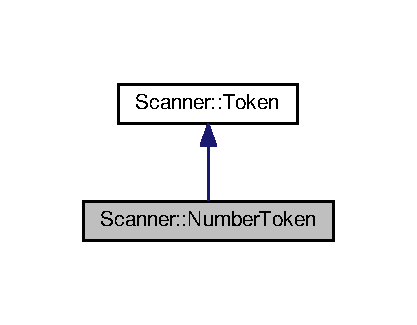
\includegraphics[width=200pt]{class_scanner_1_1_number_token__inherit__graph}
\end{center}
\end{figure}


Collaboration diagram for Scanner\+:\+:Number\+Token\+:
\nopagebreak
\begin{figure}[H]
\begin{center}
\leavevmode
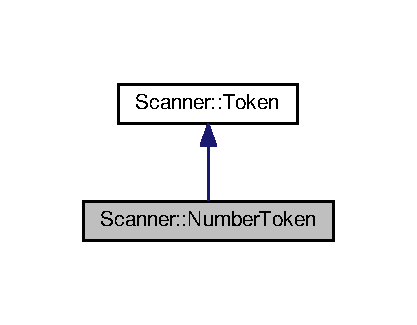
\includegraphics[width=200pt]{class_scanner_1_1_number_token__coll__graph}
\end{center}
\end{figure}
\subsection*{Public Member Functions}
\begin{DoxyCompactItemize}
\item 
virtual void {\bfseries scan\+Token} (\hyperlink{class_scanner_1_1_source_file}{Source\+File} \&r\+File)\hypertarget{class_scanner_1_1_number_token_a9e1815b574446510a45a669e6cc7c750}{}\label{class_scanner_1_1_number_token_a9e1815b574446510a45a669e6cc7c750}

\end{DoxyCompactItemize}
\subsection*{Additional Inherited Members}


The documentation for this class was generated from the following files\+:\begin{DoxyCompactItemize}
\item 
Scanner/Number\+Token.\+h\item 
Scanner/Number\+Token.\+cpp\end{DoxyCompactItemize}

\hypertarget{class_parser_1_1_parser_s_t}{}\section{Parser\+:\+:Parser\+ST Class Reference}
\label{class_parser_1_1_parser_s_t}\index{Parser\+::\+Parser\+ST@{Parser\+::\+Parser\+ST}}
\subsection*{Public Member Functions}
\begin{DoxyCompactItemize}
\item 
{\bfseries Parser\+ST} (\hyperlink{class_scanner_1_1_scanner_s_t}{Scanner\+ST} \&s)\hypertarget{class_parser_1_1_parser_s_t_a9cfdf78fb5d71c26da23849566018cfb}{}\label{class_parser_1_1_parser_s_t_a9cfdf78fb5d71c26da23849566018cfb}

\item 
void \hyperlink{class_parser_1_1_parser_s_t_a16f3b01f13e45b17388cdd735ff5a116}{parse} ()
\begin{DoxyCompactList}\small\item\em Generates the parse tree. \end{DoxyCompactList}\item 
{\bfseries Parser\+ST} (\hyperlink{class_scanner_1_1_scanner_s_t}{Scanner\+ST} \&s)\hypertarget{class_parser_1_1_parser_s_t_a9cfdf78fb5d71c26da23849566018cfb}{}\label{class_parser_1_1_parser_s_t_a9cfdf78fb5d71c26da23849566018cfb}

\item 
void {\bfseries parse} ()\hypertarget{class_parser_1_1_parser_s_t_a16f3b01f13e45b17388cdd735ff5a116}{}\label{class_parser_1_1_parser_s_t_a16f3b01f13e45b17388cdd735ff5a116}

\end{DoxyCompactItemize}


\subsection{Member Function Documentation}
\index{Parser\+::\+Parser\+ST@{Parser\+::\+Parser\+ST}!parse@{parse}}
\index{parse@{parse}!Parser\+::\+Parser\+ST@{Parser\+::\+Parser\+ST}}
\subsubsection[{\texorpdfstring{parse()}{parse()}}]{\setlength{\rightskip}{0pt plus 5cm}void Parser\+::\+Parser\+S\+T\+::parse (
\begin{DoxyParamCaption}
{}
\end{DoxyParamCaption}
)}\hypertarget{class_parser_1_1_parser_s_t_a16f3b01f13e45b17388cdd735ff5a116}{}\label{class_parser_1_1_parser_s_t_a16f3b01f13e45b17388cdd735ff5a116}


Generates the parse tree. 


\begin{DoxyParams}{Parameters}
{\em None} & \\
\hline
\end{DoxyParams}
\begin{DoxyReturn}{Returns}
Void. 
\end{DoxyReturn}


The documentation for this class was generated from the following files\+:\begin{DoxyCompactItemize}
\item 
Parser/Parser\+S\+T.\+h\item 
Parser/Parser\+S\+T.\+cpp\end{DoxyCompactItemize}

\hypertarget{class_parser_1_1_parser_test}{}\section{Parser\+:\+:Parser\+Test Class Reference}
\label{class_parser_1_1_parser_test}\index{Parser\+::\+Parser\+Test@{Parser\+::\+Parser\+Test}}


Inheritance diagram for Parser\+:\+:Parser\+Test\+:
\nopagebreak
\begin{figure}[H]
\begin{center}
\leavevmode
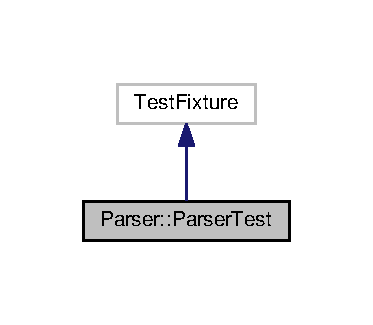
\includegraphics[width=179pt]{class_parser_1_1_parser_test__inherit__graph}
\end{center}
\end{figure}


Collaboration diagram for Parser\+:\+:Parser\+Test\+:
\nopagebreak
\begin{figure}[H]
\begin{center}
\leavevmode
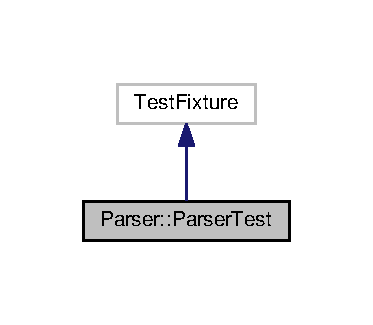
\includegraphics[width=179pt]{class_parser_1_1_parser_test__coll__graph}
\end{center}
\end{figure}
\subsection*{Public Member Functions}
\begin{DoxyCompactItemize}
\item 
void {\bfseries set\+Up} ()\hypertarget{class_parser_1_1_parser_test_ad371c6d0d9cc1093002f30f2829fd13a}{}\label{class_parser_1_1_parser_test_ad371c6d0d9cc1093002f30f2829fd13a}

\item 
void {\bfseries tear\+Down} ()\hypertarget{class_parser_1_1_parser_test_a500f9c38b4ce0decb9a0179f885561f3}{}\label{class_parser_1_1_parser_test_a500f9c38b4ce0decb9a0179f885561f3}

\end{DoxyCompactItemize}
\subsection*{Static Public Member Functions}
\begin{DoxyCompactItemize}
\item 
static Cpp\+Unit\+::\+Test $\ast$ {\bfseries suite} ()\hypertarget{class_parser_1_1_parser_test_a88132fa6757e8d419275ab7203c35696}{}\label{class_parser_1_1_parser_test_a88132fa6757e8d419275ab7203c35696}

\end{DoxyCompactItemize}
\subsection*{Protected Member Functions}
\begin{DoxyCompactItemize}
\item 
void {\bfseries test\+Tree\+Node} ()\hypertarget{class_parser_1_1_parser_test_aa147dba70e45393c0b18fd3abc10cd3c}{}\label{class_parser_1_1_parser_test_aa147dba70e45393c0b18fd3abc10cd3c}

\end{DoxyCompactItemize}


The documentation for this class was generated from the following files\+:\begin{DoxyCompactItemize}
\item 
Parser\+Test/Parser\+Test.\+h\item 
Parser\+Test/Parser\+Test.\+cpp\end{DoxyCompactItemize}

\hypertarget{class_scanner_1_1_scanner_s_t}{}\section{Scanner\+:\+:Scanner\+ST Class Reference}
\label{class_scanner_1_1_scanner_s_t}\index{Scanner\+::\+Scanner\+ST@{Scanner\+::\+Scanner\+ST}}
\subsection*{Public Member Functions}
\begin{DoxyCompactItemize}
\item 
{\bfseries Scanner\+ST} (\hyperlink{class_scanner_1_1_source_file}{Source\+File} \&r\+File)\hypertarget{class_scanner_1_1_scanner_s_t_af1cd26d3ff05ae3183adbdbf2d8f4392}{}\label{class_scanner_1_1_scanner_s_t_af1cd26d3ff05ae3183adbdbf2d8f4392}

\item 
void {\bfseries cur\+Token} (\hyperlink{class_scanner_1_1_token}{Token} \&t)\hypertarget{class_scanner_1_1_scanner_s_t_a63aa26d0733a3f7f8fdd8f15411246b6}{}\label{class_scanner_1_1_scanner_s_t_a63aa26d0733a3f7f8fdd8f15411246b6}

\item 
void {\bfseries next\+Token} (\hyperlink{class_scanner_1_1_token}{Token} \&t)\hypertarget{class_scanner_1_1_scanner_s_t_a1a27e8bad6b20e84c9b4dc383347cb91}{}\label{class_scanner_1_1_scanner_s_t_a1a27e8bad6b20e84c9b4dc383347cb91}

\item 
std\+::shared\+\_\+ptr$<$ \hyperlink{class_scanner_1_1_token}{Token} $>$ {\bfseries scan} ()\hypertarget{class_scanner_1_1_scanner_s_t_add144d55d63a342f3f5d2d40062551d1}{}\label{class_scanner_1_1_scanner_s_t_add144d55d63a342f3f5d2d40062551d1}

\end{DoxyCompactItemize}
\subsection*{Protected Member Functions}
\begin{DoxyCompactItemize}
\item 
void {\bfseries skip\+White\+Space} ()\hypertarget{class_scanner_1_1_scanner_s_t_a6f48ab6824e8d82e84a51e6aa5d54d38}{}\label{class_scanner_1_1_scanner_s_t_a6f48ab6824e8d82e84a51e6aa5d54d38}

\end{DoxyCompactItemize}


The documentation for this class was generated from the following files\+:\begin{DoxyCompactItemize}
\item 
Scanner/Scanner\+S\+T.\+h\item 
Scanner/Scanner\+S\+T.\+cpp\end{DoxyCompactItemize}

\hypertarget{class_scanner_1_1_scanner_test}{}\section{Scanner\+:\+:Scanner\+Test Class Reference}
\label{class_scanner_1_1_scanner_test}\index{Scanner\+::\+Scanner\+Test@{Scanner\+::\+Scanner\+Test}}


Inheritance diagram for Scanner\+:\+:Scanner\+Test\+:
\nopagebreak
\begin{figure}[H]
\begin{center}
\leavevmode
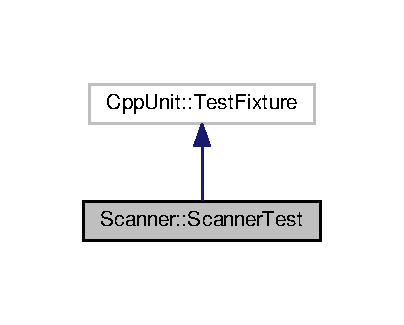
\includegraphics[width=194pt]{class_scanner_1_1_scanner_test__inherit__graph}
\end{center}
\end{figure}


Collaboration diagram for Scanner\+:\+:Scanner\+Test\+:
\nopagebreak
\begin{figure}[H]
\begin{center}
\leavevmode
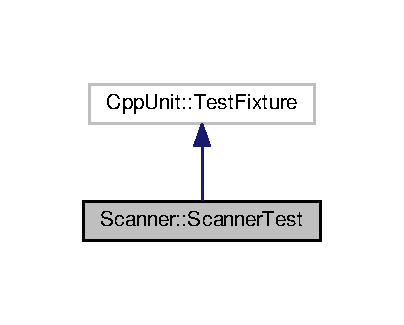
\includegraphics[width=194pt]{class_scanner_1_1_scanner_test__coll__graph}
\end{center}
\end{figure}
\subsection*{Public Member Functions}
\begin{DoxyCompactItemize}
\item 
void {\bfseries set\+Up} ()\hypertarget{class_scanner_1_1_scanner_test_af1f15a7f621e57f485d905c912ff4669}{}\label{class_scanner_1_1_scanner_test_af1f15a7f621e57f485d905c912ff4669}

\item 
void {\bfseries tear\+Down} ()\hypertarget{class_scanner_1_1_scanner_test_a72e53c25dffb1a798a76c3076c1126de}{}\label{class_scanner_1_1_scanner_test_a72e53c25dffb1a798a76c3076c1126de}

\end{DoxyCompactItemize}
\subsection*{Static Public Member Functions}
\begin{DoxyCompactItemize}
\item 
static Cpp\+Unit\+::\+Test $\ast$ {\bfseries suite} ()\hypertarget{class_scanner_1_1_scanner_test_a8259a1f3d89271f51bbadba89bd32395}{}\label{class_scanner_1_1_scanner_test_a8259a1f3d89271f51bbadba89bd32395}

\end{DoxyCompactItemize}
\subsection*{Protected Member Functions}
\begin{DoxyCompactItemize}
\item 
void {\bfseries test\+Source\+File} ()\hypertarget{class_scanner_1_1_scanner_test_aa322e116bb9ea87b9de421b4b48541ed}{}\label{class_scanner_1_1_scanner_test_aa322e116bb9ea87b9de421b4b48541ed}

\item 
void {\bfseries test\+Scan\+Token} ()\hypertarget{class_scanner_1_1_scanner_test_aefc9257a6d9d9f77bf6d9d67eec8fb48}{}\label{class_scanner_1_1_scanner_test_aefc9257a6d9d9f77bf6d9d67eec8fb48}

\end{DoxyCompactItemize}


The documentation for this class was generated from the following files\+:\begin{DoxyCompactItemize}
\item 
Scanner\+Test/Scanner\+Test.\+h\item 
Scanner\+Test/Scanner\+Test.\+cpp\end{DoxyCompactItemize}

\hypertarget{class_scanner_1_1_source_file}{}\section{Scanner\+:\+:Source\+File Class Reference}
\label{class_scanner_1_1_source_file}\index{Scanner\+::\+Source\+File@{Scanner\+::\+Source\+File}}


{\ttfamily \#include $<$Source\+File.\+h$>$}

\subsection*{Public Member Functions}
\begin{DoxyCompactItemize}
\item 
\hyperlink{class_scanner_1_1_source_file_a69413a98a0eff1311709148adfc0f222}{Source\+File} ()
\item 
virtual \hyperlink{class_scanner_1_1_source_file_a6284afa603e0dd8fbbd39ef3f3a5f6e8}{$\sim$\+Source\+File} ()
\item 
bool \hyperlink{class_scanner_1_1_source_file_a9eebbc5f778162566288961966df398c}{init} (const std\+::string \&src\+File\+Name)
\item 
int \hyperlink{class_scanner_1_1_source_file_a919d7efa693790e75e7051fc67479e34}{get\+Line\+Num} ()
\item 
int \hyperlink{class_scanner_1_1_source_file_a3e0efd4171c7225474bf1d9c5f5a8299}{get\+Col\+Num} ()
\item 
char \hyperlink{class_scanner_1_1_source_file_ac6f02448138ec25c4e8e338d645ea256}{peek\+Char} ()
\item 
char \hyperlink{class_scanner_1_1_source_file_a7592182b0200b3f095ad6642ce2f6092}{next\+Char} ()
\item 
char \hyperlink{class_scanner_1_1_source_file_a5ef11af7fec78f07581a071d631dd64d}{cur\+Char} ()
\end{DoxyCompactItemize}


\subsection{Constructor \& Destructor Documentation}
\index{Scanner\+::\+Source\+File@{Scanner\+::\+Source\+File}!Source\+File@{Source\+File}}
\index{Source\+File@{Source\+File}!Scanner\+::\+Source\+File@{Scanner\+::\+Source\+File}}
\subsubsection[{\texorpdfstring{Source\+File()}{SourceFile()}}]{\setlength{\rightskip}{0pt plus 5cm}Scanner\+::\+Source\+File\+::\+Source\+File (
\begin{DoxyParamCaption}
{}
\end{DoxyParamCaption}
)}\hypertarget{class_scanner_1_1_source_file_a69413a98a0eff1311709148adfc0f222}{}\label{class_scanner_1_1_source_file_a69413a98a0eff1311709148adfc0f222}
\index{Scanner\+::\+Source\+File@{Scanner\+::\+Source\+File}!````~Source\+File@{$\sim$\+Source\+File}}
\index{````~Source\+File@{$\sim$\+Source\+File}!Scanner\+::\+Source\+File@{Scanner\+::\+Source\+File}}
\subsubsection[{\texorpdfstring{$\sim$\+Source\+File()}{~SourceFile()}}]{\setlength{\rightskip}{0pt plus 5cm}Scanner\+::\+Source\+File\+::$\sim$\+Source\+File (
\begin{DoxyParamCaption}
{}
\end{DoxyParamCaption}
)\hspace{0.3cm}{\ttfamily [virtual]}}\hypertarget{class_scanner_1_1_source_file_a6284afa603e0dd8fbbd39ef3f3a5f6e8}{}\label{class_scanner_1_1_source_file_a6284afa603e0dd8fbbd39ef3f3a5f6e8}


\subsection{Member Function Documentation}
\index{Scanner\+::\+Source\+File@{Scanner\+::\+Source\+File}!cur\+Char@{cur\+Char}}
\index{cur\+Char@{cur\+Char}!Scanner\+::\+Source\+File@{Scanner\+::\+Source\+File}}
\subsubsection[{\texorpdfstring{cur\+Char()}{curChar()}}]{\setlength{\rightskip}{0pt plus 5cm}char Scanner\+::\+Source\+File\+::cur\+Char (
\begin{DoxyParamCaption}
{}
\end{DoxyParamCaption}
)}\hypertarget{class_scanner_1_1_source_file_a5ef11af7fec78f07581a071d631dd64d}{}\label{class_scanner_1_1_source_file_a5ef11af7fec78f07581a071d631dd64d}
\index{Scanner\+::\+Source\+File@{Scanner\+::\+Source\+File}!get\+Col\+Num@{get\+Col\+Num}}
\index{get\+Col\+Num@{get\+Col\+Num}!Scanner\+::\+Source\+File@{Scanner\+::\+Source\+File}}
\subsubsection[{\texorpdfstring{get\+Col\+Num()}{getColNum()}}]{\setlength{\rightskip}{0pt plus 5cm}int Scanner\+::\+Source\+File\+::get\+Col\+Num (
\begin{DoxyParamCaption}
{}
\end{DoxyParamCaption}
)\hspace{0.3cm}{\ttfamily [inline]}}\hypertarget{class_scanner_1_1_source_file_a3e0efd4171c7225474bf1d9c5f5a8299}{}\label{class_scanner_1_1_source_file_a3e0efd4171c7225474bf1d9c5f5a8299}
\index{Scanner\+::\+Source\+File@{Scanner\+::\+Source\+File}!get\+Line\+Num@{get\+Line\+Num}}
\index{get\+Line\+Num@{get\+Line\+Num}!Scanner\+::\+Source\+File@{Scanner\+::\+Source\+File}}
\subsubsection[{\texorpdfstring{get\+Line\+Num()}{getLineNum()}}]{\setlength{\rightskip}{0pt plus 5cm}int Scanner\+::\+Source\+File\+::get\+Line\+Num (
\begin{DoxyParamCaption}
{}
\end{DoxyParamCaption}
)\hspace{0.3cm}{\ttfamily [inline]}}\hypertarget{class_scanner_1_1_source_file_a919d7efa693790e75e7051fc67479e34}{}\label{class_scanner_1_1_source_file_a919d7efa693790e75e7051fc67479e34}
\index{Scanner\+::\+Source\+File@{Scanner\+::\+Source\+File}!init@{init}}
\index{init@{init}!Scanner\+::\+Source\+File@{Scanner\+::\+Source\+File}}
\subsubsection[{\texorpdfstring{init(const std\+::string \&src\+File\+Name)}{init(const std::string &srcFileName)}}]{\setlength{\rightskip}{0pt plus 5cm}bool Scanner\+::\+Source\+File\+::init (
\begin{DoxyParamCaption}
\item[{const std\+::string \&}]{src\+File\+Name}
\end{DoxyParamCaption}
)}\hypertarget{class_scanner_1_1_source_file_a9eebbc5f778162566288961966df398c}{}\label{class_scanner_1_1_source_file_a9eebbc5f778162566288961966df398c}
\index{Scanner\+::\+Source\+File@{Scanner\+::\+Source\+File}!next\+Char@{next\+Char}}
\index{next\+Char@{next\+Char}!Scanner\+::\+Source\+File@{Scanner\+::\+Source\+File}}
\subsubsection[{\texorpdfstring{next\+Char()}{nextChar()}}]{\setlength{\rightskip}{0pt plus 5cm}char Scanner\+::\+Source\+File\+::next\+Char (
\begin{DoxyParamCaption}
{}
\end{DoxyParamCaption}
)}\hypertarget{class_scanner_1_1_source_file_a7592182b0200b3f095ad6642ce2f6092}{}\label{class_scanner_1_1_source_file_a7592182b0200b3f095ad6642ce2f6092}
\index{Scanner\+::\+Source\+File@{Scanner\+::\+Source\+File}!peek\+Char@{peek\+Char}}
\index{peek\+Char@{peek\+Char}!Scanner\+::\+Source\+File@{Scanner\+::\+Source\+File}}
\subsubsection[{\texorpdfstring{peek\+Char()}{peekChar()}}]{\setlength{\rightskip}{0pt plus 5cm}char Scanner\+::\+Source\+File\+::peek\+Char (
\begin{DoxyParamCaption}
{}
\end{DoxyParamCaption}
)}\hypertarget{class_scanner_1_1_source_file_ac6f02448138ec25c4e8e338d645ea256}{}\label{class_scanner_1_1_source_file_ac6f02448138ec25c4e8e338d645ea256}


The documentation for this class was generated from the following files\+:\begin{DoxyCompactItemize}
\item 
/home/vagrant/\+Projects/\+Smart\+Controller/\+Smart\+Compiler/\+Scanner/\hyperlink{_source_file_8h}{Source\+File.\+h}\item 
/home/vagrant/\+Projects/\+Smart\+Controller/\+Smart\+Compiler/\+Scanner/\hyperlink{_source_file_8cpp}{Source\+File.\+cpp}\end{DoxyCompactItemize}

\hypertarget{class_scanner_1_1_special_symbol_token}{}\section{Scanner\+:\+:Special\+Symbol\+Token Class Reference}
\label{class_scanner_1_1_special_symbol_token}\index{Scanner\+::\+Special\+Symbol\+Token@{Scanner\+::\+Special\+Symbol\+Token}}


Inheritance diagram for Scanner\+:\+:Special\+Symbol\+Token\+:
\nopagebreak
\begin{figure}[H]
\begin{center}
\leavevmode
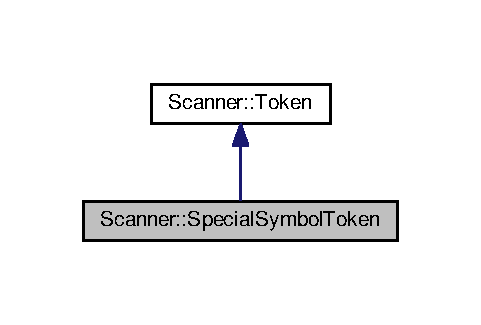
\includegraphics[width=231pt]{class_scanner_1_1_special_symbol_token__inherit__graph}
\end{center}
\end{figure}


Collaboration diagram for Scanner\+:\+:Special\+Symbol\+Token\+:
\nopagebreak
\begin{figure}[H]
\begin{center}
\leavevmode
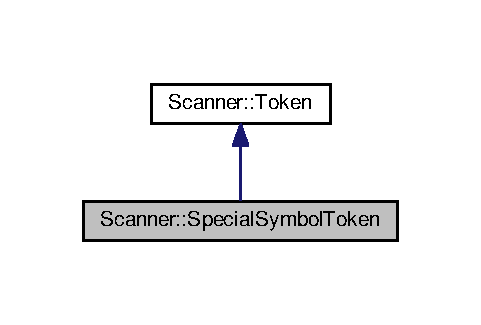
\includegraphics[width=231pt]{class_scanner_1_1_special_symbol_token__coll__graph}
\end{center}
\end{figure}
\subsection*{Public Member Functions}
\begin{DoxyCompactItemize}
\item 
virtual void {\bfseries scan\+Token} (\hyperlink{class_scanner_1_1_source_file}{Source\+File} \&r\+File)\hypertarget{class_scanner_1_1_special_symbol_token_a6f4ce9fb7bdb49c11400f41a9aef1030}{}\label{class_scanner_1_1_special_symbol_token_a6f4ce9fb7bdb49c11400f41a9aef1030}

\end{DoxyCompactItemize}
\subsection*{Additional Inherited Members}


The documentation for this class was generated from the following files\+:\begin{DoxyCompactItemize}
\item 
Scanner/Special\+Symbol\+Token.\+h\item 
Scanner/Special\+Symbol\+Token.\+cpp\end{DoxyCompactItemize}

\hypertarget{class_scanner_1_1_token}{}\section{Scanner\+:\+:Token Class Reference}
\label{class_scanner_1_1_token}\index{Scanner\+::\+Token@{Scanner\+::\+Token}}


Inheritance diagram for Scanner\+:\+:Token\+:
\nopagebreak
\begin{figure}[H]
\begin{center}
\leavevmode
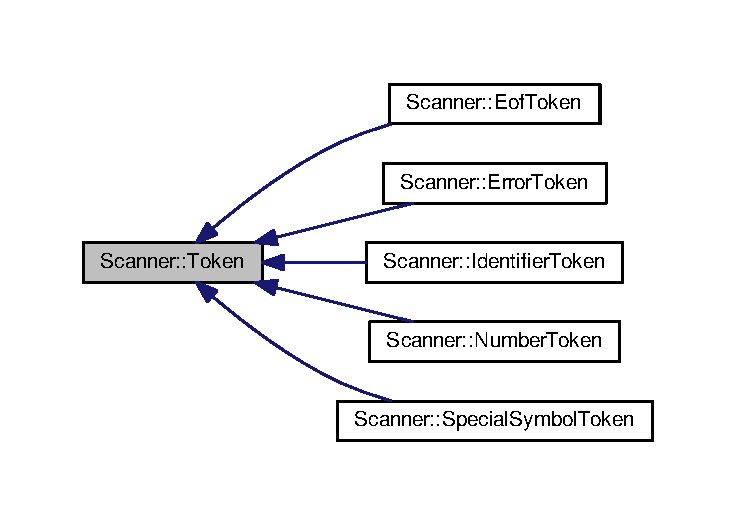
\includegraphics[width=350pt]{class_scanner_1_1_token__inherit__graph}
\end{center}
\end{figure}
\subsection*{Public Types}
\begin{DoxyCompactItemize}
\item 
enum {\bfseries E\+Token\+Type} \+: uint \{ \\*
{\bfseries E\+R\+R\+OR} = 0, 
{\bfseries E\+N\+D\+\_\+\+O\+F\+\_\+\+F\+I\+LE}, 
{\bfseries I\+D\+E\+N\+T\+I\+F\+I\+ER}, 
{\bfseries P\+R\+O\+G\+R\+AM}, 
\\*
{\bfseries E\+N\+D\+\_\+\+P\+R\+O\+G\+R\+AM}, 
{\bfseries V\+AR}, 
{\bfseries E\+N\+D\+\_\+\+V\+AR}, 
{\bfseries C\+O\+L\+O\+N\+\_\+\+S\+YM}, 
\\*
{\bfseries A\+S\+S\+I\+G\+N\+\_\+\+S\+YM}, 
{\bfseries S\+E\+M\+I\+C\+O\+L\+\_\+\+S\+YM}, 
{\bfseries P\+E\+R\+C\+E\+N\+T\+\_\+\+S\+YM}, 
{\bfseries P\+E\+R\+I\+O\+D\+\_\+\+S\+YM}, 
\\*
{\bfseries U\+N\+K\+N\+O\+WN}
 \}\hypertarget{class_scanner_1_1_token_adba36ae34c8f4befddcbc76c761cc244}{}\label{class_scanner_1_1_token_adba36ae34c8f4befddcbc76c761cc244}

\end{DoxyCompactItemize}
\subsection*{Public Member Functions}
\begin{DoxyCompactItemize}
\item 
virtual void {\bfseries scan\+Token} (\hyperlink{class_scanner_1_1_source_file}{Source\+File} \&r\+File)\hypertarget{class_scanner_1_1_token_a8a05ceeb54beba7a7212564b4f164446}{}\label{class_scanner_1_1_token_a8a05ceeb54beba7a7212564b4f164446}

\item 
E\+Token\+Type {\bfseries get\+Type} ()\hypertarget{class_scanner_1_1_token_ab1b8fca3f87cdb8d94d689bea15c9ad6}{}\label{class_scanner_1_1_token_ab1b8fca3f87cdb8d94d689bea15c9ad6}

\item 
std\+::string {\bfseries get\+Text} ()\hypertarget{class_scanner_1_1_token_a2154667730517a87309c8ca9e81552e3}{}\label{class_scanner_1_1_token_a2154667730517a87309c8ca9e81552e3}

\item 
int {\bfseries get\+Line} ()\hypertarget{class_scanner_1_1_token_a8da596b64a487ea98244ae269cda90d3}{}\label{class_scanner_1_1_token_a8da596b64a487ea98244ae269cda90d3}

\item 
int {\bfseries get\+Col} ()\hypertarget{class_scanner_1_1_token_a55e7d1b5e89057371ac3924b9cd3708b}{}\label{class_scanner_1_1_token_a55e7d1b5e89057371ac3924b9cd3708b}

\end{DoxyCompactItemize}
\subsection*{Static Public Member Functions}
\begin{DoxyCompactItemize}
\item 
static E\+Token\+Type {\bfseries text2\+Type} (const std\+::string \&some\+Text)\hypertarget{class_scanner_1_1_token_a9d998150939f8ef7fcd0a50f6bece5d8}{}\label{class_scanner_1_1_token_a9d998150939f8ef7fcd0a50f6bece5d8}

\item 
static bool {\bfseries is\+Key\+Word} (const std\+::string \&some\+Text)\hypertarget{class_scanner_1_1_token_a76634cafc7a564d36533376a8ee58f58}{}\label{class_scanner_1_1_token_a76634cafc7a564d36533376a8ee58f58}

\item 
static bool {\bfseries is\+Special\+Symbol} (const std\+::string \&some\+Text)\hypertarget{class_scanner_1_1_token_adc64dc5bb8e26e9b238ac940395826f3}{}\label{class_scanner_1_1_token_adc64dc5bb8e26e9b238ac940395826f3}

\end{DoxyCompactItemize}
\subsection*{Static Public Attributes}
\begin{DoxyCompactItemize}
\item 
static const std\+::vector$<$ std\+::string $>$ {\bfseries Token\+Text}
\item 
static const std\+::vector$<$ E\+Token\+Type $>$ {\bfseries Key\+Words}
\item 
static const std\+::vector$<$ E\+Token\+Type $>$ {\bfseries Special\+Symbols}
\end{DoxyCompactItemize}
\subsection*{Protected Attributes}
\begin{DoxyCompactItemize}
\item 
E\+Token\+Type {\bfseries m\+\_\+token\+Type}\hypertarget{class_scanner_1_1_token_afdb4cd3121e353221f190997dd20648f}{}\label{class_scanner_1_1_token_afdb4cd3121e353221f190997dd20648f}

\item 
std\+::string {\bfseries m\+\_\+token\+Text}\hypertarget{class_scanner_1_1_token_a03cda26b93d4751fe631c65912e6d446}{}\label{class_scanner_1_1_token_a03cda26b93d4751fe631c65912e6d446}

\item 
int {\bfseries m\+\_\+line\+Num}\hypertarget{class_scanner_1_1_token_a00d8f8fc6715651a1a02e11579ce099f}{}\label{class_scanner_1_1_token_a00d8f8fc6715651a1a02e11579ce099f}

\item 
int {\bfseries m\+\_\+col\+Num}\hypertarget{class_scanner_1_1_token_a34c62ba179be0a9881fe5fb0c38f89b1}{}\label{class_scanner_1_1_token_a34c62ba179be0a9881fe5fb0c38f89b1}

\end{DoxyCompactItemize}


\subsection{Member Data Documentation}
\index{Scanner\+::\+Token@{Scanner\+::\+Token}!Key\+Words@{Key\+Words}}
\index{Key\+Words@{Key\+Words}!Scanner\+::\+Token@{Scanner\+::\+Token}}
\subsubsection[{\texorpdfstring{Key\+Words}{KeyWords}}]{\setlength{\rightskip}{0pt plus 5cm}const std\+::vector$<$ Token\+::\+E\+Token\+Type $>$ Scanner\+::\+Token\+::\+Key\+Words\hspace{0.3cm}{\ttfamily [static]}}\hypertarget{class_scanner_1_1_token_ac3bfa7f186802c0fac1dbbcc379b4978}{}\label{class_scanner_1_1_token_ac3bfa7f186802c0fac1dbbcc379b4978}
{\bfseries Initial value\+:}
\begin{DoxyCode}
=
\{
    ETokenType::PROGRAM,
    ETokenType::END\_PROGRAM,
    ETokenType::VAR,
    ETokenType::END\_VAR,
\}
\end{DoxyCode}
\index{Scanner\+::\+Token@{Scanner\+::\+Token}!Special\+Symbols@{Special\+Symbols}}
\index{Special\+Symbols@{Special\+Symbols}!Scanner\+::\+Token@{Scanner\+::\+Token}}
\subsubsection[{\texorpdfstring{Special\+Symbols}{SpecialSymbols}}]{\setlength{\rightskip}{0pt plus 5cm}const std\+::vector$<$ Token\+::\+E\+Token\+Type $>$ Scanner\+::\+Token\+::\+Special\+Symbols\hspace{0.3cm}{\ttfamily [static]}}\hypertarget{class_scanner_1_1_token_a717646234da005d9ccb185c1f782afd1}{}\label{class_scanner_1_1_token_a717646234da005d9ccb185c1f782afd1}
{\bfseries Initial value\+:}
\begin{DoxyCode}
=
\{
    ETokenType::COLON\_SYM,
    ETokenType::ASSIGN\_SYM,
    ETokenType::SEMICOL\_SYM,
    ETokenType::PERCENT\_SYM,
    ETokenType::PERIOD\_SYM,
\}
\end{DoxyCode}
\index{Scanner\+::\+Token@{Scanner\+::\+Token}!Token\+Text@{Token\+Text}}
\index{Token\+Text@{Token\+Text}!Scanner\+::\+Token@{Scanner\+::\+Token}}
\subsubsection[{\texorpdfstring{Token\+Text}{TokenText}}]{\setlength{\rightskip}{0pt plus 5cm}const std\+::vector$<$ std\+::string $>$ Scanner\+::\+Token\+::\+Token\+Text\hspace{0.3cm}{\ttfamily [static]}}\hypertarget{class_scanner_1_1_token_a01fb9e95d9a1c93f3e6adf3ea208bf36}{}\label{class_scanner_1_1_token_a01fb9e95d9a1c93f3e6adf3ea208bf36}
{\bfseries Initial value\+:}
\begin{DoxyCode}
=
\{
    \textcolor{stringliteral}{"ERROR"},
    \textcolor{stringliteral}{"END\_OF\_FILE"},
    \textcolor{stringliteral}{"IDENTIFIER"},
    \textcolor{stringliteral}{"PROGRAM"},
    \textcolor{stringliteral}{"END\_PROGRAM"},
    \textcolor{stringliteral}{"VAR"},
    \textcolor{stringliteral}{"END\_VAR"},
    \textcolor{stringliteral}{":"},
    \textcolor{stringliteral}{":="},
    \textcolor{stringliteral}{";"},
    \textcolor{stringliteral}{"%"},
    \textcolor{stringliteral}{"."},
    \textcolor{stringliteral}{"UNKNOWN"},
\}
\end{DoxyCode}


The documentation for this class was generated from the following files\+:\begin{DoxyCompactItemize}
\item 
Scanner/Token.\+h\item 
Scanner/Token.\+cpp\end{DoxyCompactItemize}

\hypertarget{class_parser_1_1_tree_node}{}\section{Parser\+:\+:Tree\+Node Class Reference}
\label{class_parser_1_1_tree_node}\index{Parser\+::\+Tree\+Node@{Parser\+::\+Tree\+Node}}
\subsection*{Public Types}
\begin{DoxyCompactItemize}
\item 
enum {\bfseries E\+Node\+Type} \+: uint \{ \\*
{\bfseries E\+R\+R\+OR} = 0, 
{\bfseries P\+R\+O\+G\+R\+AM}, 
{\bfseries F\+U\+N\+C\+T\+I\+ON}, 
{\bfseries A\+S\+S\+G\+N\+\_\+\+S\+T\+A\+T\+EM}, 
\\*
{\bfseries E\+Q\+\_\+\+OP}, 
{\bfseries N\+O\+T\+\_\+\+OP}, 
{\bfseries A\+D\+D\+\_\+\+OP}, 
{\bfseries S\+U\+B\+\_\+\+OP}, 
\\*
{\bfseries M\+U\+L\+\_\+\+OP}, 
{\bfseries D\+I\+V\+\_\+\+OP}, 
{\bfseries V\+A\+R\+\_\+\+O\+PR}, 
{\bfseries U\+N\+K\+N\+O\+WN}
 \}\hypertarget{class_parser_1_1_tree_node_ac4fbe01974a5f95dfc45c6deea2fd171}{}\label{class_parser_1_1_tree_node_ac4fbe01974a5f95dfc45c6deea2fd171}

\item 
enum {\bfseries E\+Token\+Type} \+: uint \{ \\*
{\bfseries E\+R\+R\+OR} = 0, 
{\bfseries P\+R\+O\+G\+R\+AM}, 
{\bfseries F\+U\+N\+C\+T\+I\+ON}, 
{\bfseries A\+S\+S\+G\+N\+\_\+\+S\+T\+A\+T\+EM}, 
\\*
{\bfseries E\+Q\+\_\+\+OP}, 
{\bfseries N\+O\+T\+\_\+\+OP}, 
{\bfseries A\+D\+D\+\_\+\+OP}, 
{\bfseries S\+U\+B\+\_\+\+OP}, 
\\*
{\bfseries M\+U\+L\+\_\+\+OP}, 
{\bfseries D\+I\+V\+\_\+\+OP}, 
{\bfseries V\+A\+R\+\_\+\+O\+PR}, 
{\bfseries U\+N\+K\+N\+O\+WN}
 \}\hypertarget{class_parser_1_1_tree_node_a8e1fc3952088b5c2b4307b6292e8ee94}{}\label{class_parser_1_1_tree_node_a8e1fc3952088b5c2b4307b6292e8ee94}

\end{DoxyCompactItemize}
\subsection*{Public Member Functions}
\begin{DoxyCompactItemize}
\item 
{\bfseries Tree\+Node} (E\+Node\+Type e, std\+::shared\+\_\+ptr$<$ \hyperlink{class_parser_1_1_tree_node}{Tree\+Node} $>$ p)\hypertarget{class_parser_1_1_tree_node_ae91b0ab18a928beb625f92fcdecd5c7b}{}\label{class_parser_1_1_tree_node_ae91b0ab18a928beb625f92fcdecd5c7b}

\item 
void {\bfseries add\+Child} (std\+::string name, std\+::shared\+\_\+ptr$<$ \hyperlink{class_parser_1_1_tree_node}{Tree\+Node} $>$ c)\hypertarget{class_parser_1_1_tree_node_a4b8435fee357fdce7876d31a935ccffd}{}\label{class_parser_1_1_tree_node_a4b8435fee357fdce7876d31a935ccffd}

\end{DoxyCompactItemize}
\subsection*{Protected Attributes}
\begin{DoxyCompactItemize}
\item 
E\+Node\+Type {\bfseries m\+\_\+node\+Type}\hypertarget{class_parser_1_1_tree_node_add5798e3cf8c66136027cc2bf0966efb}{}\label{class_parser_1_1_tree_node_add5798e3cf8c66136027cc2bf0966efb}

\item 
std\+::weak\+\_\+ptr$<$ \hyperlink{class_parser_1_1_tree_node}{Tree\+Node} $>$ {\bfseries m\+\_\+parent\+Node}\hypertarget{class_parser_1_1_tree_node_a745168207785c3e1cd12ca4205f8da53}{}\label{class_parser_1_1_tree_node_a745168207785c3e1cd12ca4205f8da53}

\item 
std\+::map$<$ std\+::string, std\+::shared\+\_\+ptr$<$ \hyperlink{class_parser_1_1_tree_node}{Tree\+Node} $>$ $>$ {\bfseries m\+\_\+child\+Map}\hypertarget{class_parser_1_1_tree_node_a9a87c47a4116da5e0d5f016afc4149e1}{}\label{class_parser_1_1_tree_node_a9a87c47a4116da5e0d5f016afc4149e1}

\item 
E\+Token\+Type {\bfseries m\+\_\+node\+Type}\hypertarget{class_parser_1_1_tree_node_a2a4e098a43880ce9c30051163aed59c8}{}\label{class_parser_1_1_tree_node_a2a4e098a43880ce9c30051163aed59c8}

\item 
std\+::weak\+\_\+ptr$<$ \hyperlink{class_parser_1_1_tree_node}{Tree\+Node} $>$ {\bfseries m\+\_\+p\+Parent}\hypertarget{class_parser_1_1_tree_node_a844c2318d0df9555f25721e47fea0ab9}{}\label{class_parser_1_1_tree_node_a844c2318d0df9555f25721e47fea0ab9}

\end{DoxyCompactItemize}


The documentation for this class was generated from the following files\+:\begin{DoxyCompactItemize}
\item 
Parser/Tree\+Node.\+h\item 
Parser/Tree\+Node.\+cpp\end{DoxyCompactItemize}

\hypertarget{class_util_1_1_util_test}{}\section{Util\+:\+:Util\+Test Class Reference}
\label{class_util_1_1_util_test}\index{Util\+::\+Util\+Test@{Util\+::\+Util\+Test}}


Inheritance diagram for Util\+:\+:Util\+Test\+:
\nopagebreak
\begin{figure}[H]
\begin{center}
\leavevmode
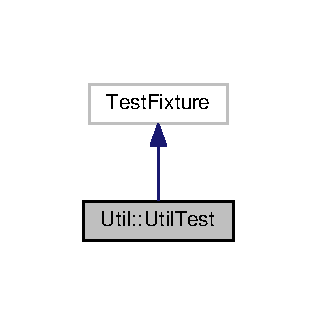
\includegraphics[width=152pt]{class_util_1_1_util_test__inherit__graph}
\end{center}
\end{figure}


Collaboration diagram for Util\+:\+:Util\+Test\+:
\nopagebreak
\begin{figure}[H]
\begin{center}
\leavevmode
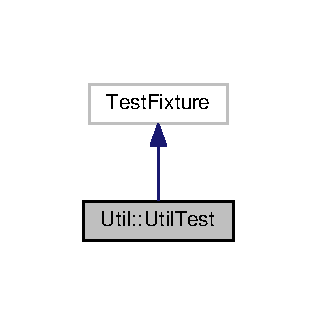
\includegraphics[width=152pt]{class_util_1_1_util_test__coll__graph}
\end{center}
\end{figure}
\subsection*{Public Member Functions}
\begin{DoxyCompactItemize}
\item 
void {\bfseries set\+Up} ()\hypertarget{class_util_1_1_util_test_a10968ee4258f61df4caa1dbba822b9e6}{}\label{class_util_1_1_util_test_a10968ee4258f61df4caa1dbba822b9e6}

\item 
void {\bfseries tear\+Down} ()\hypertarget{class_util_1_1_util_test_a0b0e3dd728dc81fc516b35ed14f7ab7e}{}\label{class_util_1_1_util_test_a0b0e3dd728dc81fc516b35ed14f7ab7e}

\end{DoxyCompactItemize}
\subsection*{Static Public Member Functions}
\begin{DoxyCompactItemize}
\item 
static Cpp\+Unit\+::\+Test $\ast$ {\bfseries suite} ()\hypertarget{class_util_1_1_util_test_a6aea16da6a30f2da7c331884402678e9}{}\label{class_util_1_1_util_test_a6aea16da6a30f2da7c331884402678e9}

\end{DoxyCompactItemize}
\subsection*{Protected Member Functions}
\begin{DoxyCompactItemize}
\item 
void {\bfseries test\+Time} ()\hypertarget{class_util_1_1_util_test_a6df1223c040166a5e42610f6ceb76666}{}\label{class_util_1_1_util_test_a6df1223c040166a5e42610f6ceb76666}

\item 
void {\bfseries test\+Message\+Mgr} ()\hypertarget{class_util_1_1_util_test_a3e88702de7b7d45377b1dc99f22bbc3a}{}\label{class_util_1_1_util_test_a3e88702de7b7d45377b1dc99f22bbc3a}

\item 
void {\bfseries test\+Config\+Reader} ()\hypertarget{class_util_1_1_util_test_ae46a726defc5ffe24f126ca1d7da3775}{}\label{class_util_1_1_util_test_ae46a726defc5ffe24f126ca1d7da3775}

\end{DoxyCompactItemize}


The documentation for this class was generated from the following files\+:\begin{DoxyCompactItemize}
\item 
Util\+Test/Util\+Test.\+h\item 
Util\+Test/Util\+Test.\+cpp\end{DoxyCompactItemize}

%--- End generated contents ---

% Index
\backmatter
\newpage
\phantomsection
\clearemptydoublepage
\addcontentsline{toc}{chapter}{Index}
\printindex

\end{document}
